\documentclass{article}
\usepackage{graphicx} % Required for inserting images
\usepackage[margin={10mm,15mm}]{geometry}
\usepackage{siunitx}
\usepackage{hyperref}
\usepackage{graphicx}
\usepackage{listings}
\usepackage{glossaries}
\usepackage{float} % 'Exactly Here' Image Positioning
\usepackage{biblatex} % Reference List
\addbibresource{references.bib}
\usepackage{amsmath} % Math
\usepackage{listings} % Code (prevents overflow!)
\usepackage{xcolor}
\usepackage{enumitem}

\title{AMME1362 Lab Report}
\author{Zev Sage}
\date{October 2026}

% Making code colourful!!!
\definecolor{codeblue}{rgb}{0.3,0.6,0.8}
\definecolor{codegray}{rgb}{0.5,0.5,0.5}
\definecolor{codeorange}{rgb}{1, 0.647, 0}
\definecolor{white}{rgb}{1,1,1}
\lstset{
    backgroundcolor=\color{white},   
    commentstyle=\color{codegray},
    keywordstyle=\color{codeorange},
    numberstyle=\tiny\color{codegray},
    stringstyle=\color{codeblue},
    basicstyle=\ttfamily\footnotesize,
    breaklines=true,                  
    numbers=left,
    showstringspaces=false
}

\begin{document}

\maketitle
\newpage

\section{Introduction}
\subsection{Background Information}
Investigating mechanical properties of materials prove essential to the field of Engineering and Science, and is integral to the function of virtually all man-made systems. Listed below are key concepts used in this investigation's analysis of four materials:
\begin{itemize}
    \item Load: The amount of Tensile force applied to a sample (proportional to stress)
    \item Gauge Length: The reference length used to calculate elongation \& strain \cite{instron_gauge_length}
    \item Engineering Stress: Defined as a ratio of the Force and initial cross-sectional area $\sigma = \frac{F}{A_0}$; three of the four mechanical properties are measures of stress
    \item Engineering Strain: Defined as the ratio of elongation to original length $\varepsilon = \frac{\Delta l}{l_0}$; one investigated property is a measure of strain
    \item Young's Modulus: Also known as Hooke's Law, it represents the slope of the elastic (linear) region of a stress-strain curve $E=\frac{\sigma}{\varepsilon}$
    \item Yield Strength: Usually defined by a $0.02\%$ strain limit, it is used as a well-defined approximation of when a material begins to undergo noticeable plastic deformation (identical in practice to the "elastic limit" where plastic deformation begins, which is difficult to evaluate) - note that for brittle substances such as acrylic, yield strength is not defined (as these materials mostly undergo elastic deformation up until fracture)
    \item Ultimate Tensile Strength: The maximum stress sustained by a material (the maximum $y$-value of a stress-strain graph)
    \item Ductility: Determined by the strain at failure (maximum strain in a stress-strain graph, provided data points after fracture are excluded), it is a measure of how well a material deforms plastically
\end{itemize}
Using Engineering Stress and Strain (which are evaluted using Load and Gauge Length respectively), this experiment will experimentally determine the Young's Modulus, Yield Strength, Ultimate Tensile Strength and Strain at Fracture of four materials.

\subsection{Aim}
The aim of this experiment is to investigate mechanical properties, including the Young's Modulus, Yield strength, Ultimate strength and Strain at Failure, of Aluminium Alloy 6061, PMMA acrylic, Mild Steel and Nylon-6.

\section{Experimental Methods}

The cross section of the chosen sample is measured (i.e. width and thickness of the sample, see Table \ref{tab:dim_table} for further information) using callipers. The sample is then loaded into a Universal Testing Machine, specimen dimensions entered, test speed set and load/displacement readings cleared before starting the test.
After fracture, the test ends; the specimen is removed, ensuring to first unload.

\begin{table}[H]
    \centering
    \begin{tabular}{ccccc}
         & Aluminium & Acrylic & Mild Steel & Nylon 6 \\
        Width ($mm$) & 12.96 & 12.71 & 12.97 & 12.77 \\
        Height ($mm$) & 2.96 & 2.91 & 2.93 & 2.87 \\
        Area ($mm^2$) & 38.36 & 30.99 & 38.00 & 36.65
    \end{tabular}
    \caption{Mean Dimensions (note, individual dimensions used for analysis)}
    \label{tab:dim_table}
\end{table}
    
\section{Results}

\begin{figure}[H]
    \centering
    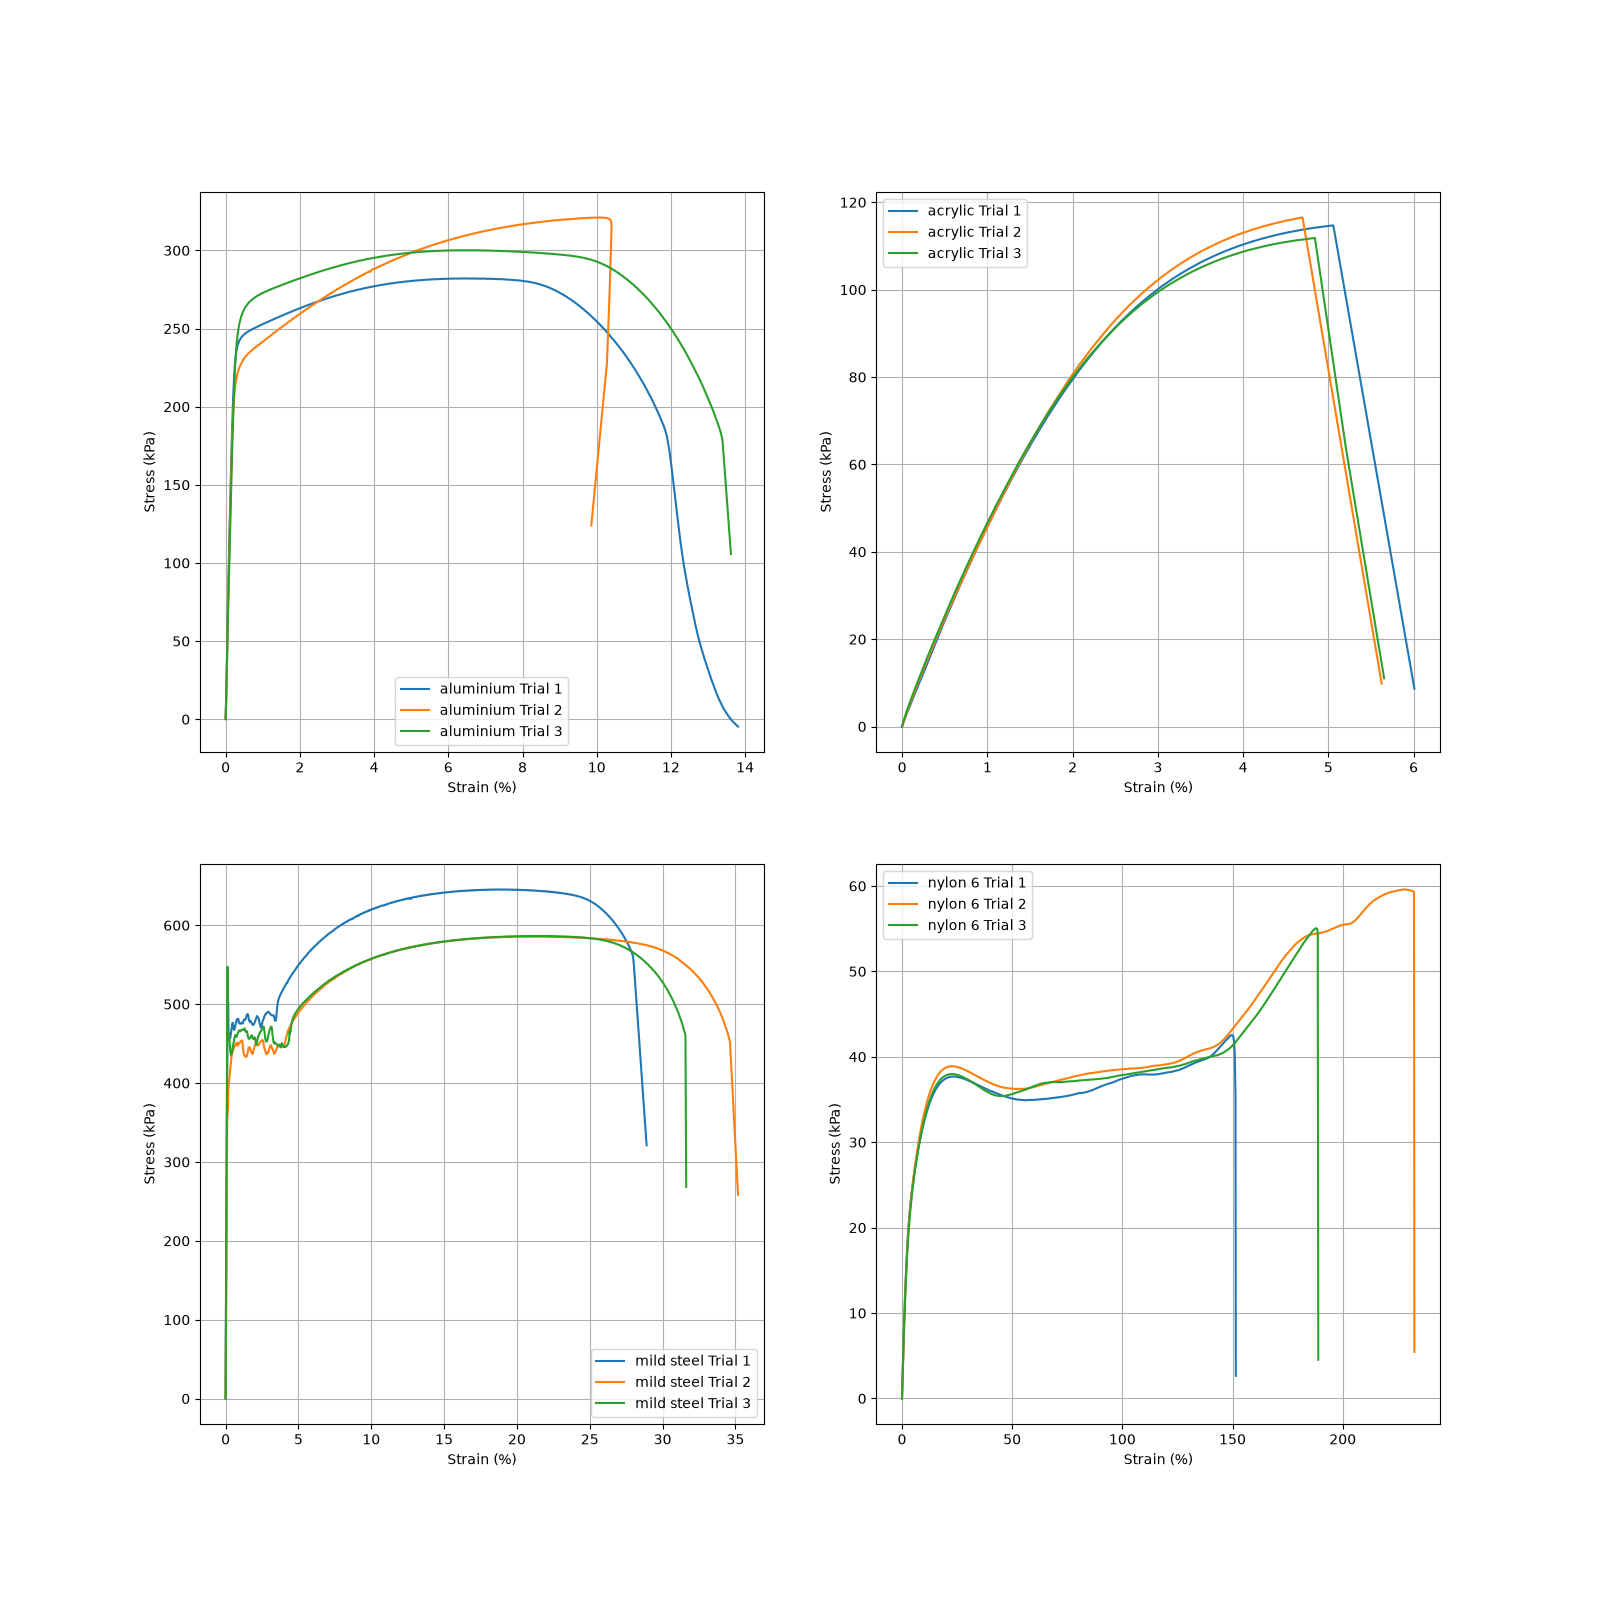
\includegraphics[width=1\textwidth]{stress_strain_graphs.png}
    \caption{Stress vs Strain for Four Materials (three trials)}
    \label{fig:stress-strain-overall}
\end{figure}

\begin{table}[H]
    \centering
    \begin{tabular}{ccccc}
         & Aluminium & Acrylic & Mild Steel & Nylon 6 \\
        Young's Modulus ($GPa$) & 74.3 & 3.58 & 374 & 0.275 \\
        Yield Strength ($MPa$) & 154 & - & 341 & 35.6 \\
        Ultimate Tensile Strength ($MPa$) & 205 & 83.5 & 419 & 39.1 \\
        Strain at Fracture & 0.119 & 0.0485 & 0.314 & 1.90 \\

    \end{tabular}
    \caption{Mean Mechanical Property Values}
    \label{tab:dim_table}
\end{table}

\subsection{Deformation \& Failure Methods}
There are two main forms of material failure - necking, and fracture; while not mutually exclusive events, the extent to which each occurs is dependent on mechanical properties (e.g. ultimate tensile strength and ductility) and its structure. On a stress vs strain graph, significant necking begins after approaching Ultimate Tensile Strength (UTS); as strain is increased further, stress is concentrated at localised deformation sites.
Mild Steel and Nylon-6's high ductility (strain at fracture) indicates more susceptibility to necking, whereas the much lower ductility of Aluminium indicates a higher susceptibility to fracturing. Acrylic, a brittle polymer, does not undergo visible plastic deformation before fracturing and so does not undergo necking.

\section{Discussion}
It was found that the highest values for Young's Modulus, Yield Strength and Ultimate Tensile Strength was that of mild steel, with mean values of $374$ GPa, $341$ MPa and $419$ MPa respectively. However, the Young's Modulus value is over $75\%$ higher than the theoretically accepted value of between $180$ and $210$ MPa (depending on type). This could be due to errors in machine calibration (e.g. with the extensometer or tensile load application) or inconsistencies within the material (such as further impurities). The Yield Strength and Ultimate Tensile Strength is relatively closer to theoretical values, however strain at fracture almost double that of theoretical values \cite{MildSteel0} \cite{MildSteel1}.

An alloy of aluminium 6061 was used in this investigation. The experimental Young's Modulus of $74.3$ GPa is $7.8\%$ higher than the theoretical value of $68.9$ GPa, which is not significant. Depending on the tempering of the alloy, the theoretical Yield Strength is around 240-280 MPa (T6) or around 110 MPa (T4); the empirically-derived Yield Strength vaules are $121$ MPa, $217$ MPa, and $124$ MPa, the second being significantly higher than the other two. The second value corresponds to the second Aluminium trial as per Figure \ref{fig:stress-strain-overall}, which demonstrates very little necking and a significantly higher tensile strength compared to the other two trials. Sources of these anomalies could be impurities, varying methods of preparation (e.g. tempering), as well as possible callibration errors. The strain at fracture varies from 12-15\% in general, demonstrated by the mean experimental value of $11.9\%$ (the second trial's noticeably less ductile behvaiour explains its somewhat lower value) \cite{Aluminium0} \cite{Aluminium1}.

The experimental values for Acrylic appear to vary little for different trials, with Young'S Modulus varying between $3.5$ GPa and $3.7$ GPa, up to $16\%$ higher than the theoretical value of $3.2$ GPa. This moderate deviation could likely be due to calibration errors or impurities, though little random error is present; instead, this could be due to preparation of the samples. The Ultimate Tensile Strength varies from $82.3$ to $84.6$ MPa, which is up to $19\%$ higher than the theoretical value of 70-71 MPa, further suggesting sample preparation as a source of systematic error or uniqueness. Finally, the experimental ductility varies between $4.7\%$ to $5\%$, lying in the accepted value range of 2-5\% \cite{Acrylic0} \cite{Acrylic1} \cite{Acrylic2}.

Interestingly, the experimental values for Nylon-6 vary significantly from experimental values. The experimental values for Young's Modulus vary from $0.272$ GPa to $0.277$ GPa - very little random error - however, they are $90\%$ below the accepted value of $3$ GPa. Furthermore, the empirical Yield Strength values vary from $30$ to $43$ MPa, about half of the accepted value of 80-85 MPa. Conversely, the Strain at Fracture empirical values vary significantly between trials from $150\%$ to $232\%$, over $250\%$ higher than the accepted value of approximately $40\%$. The lower overall tensile strength and increased ductility are likely due to measurement callibration errors and presence  impurities (such as moisture). The latter further explains the large variation in Ductility yet little variation in Yield Strength and Young's Modulus \cite{Nylon6_0} \cite{Nylon6_1}.

Overall, this experiment somewhat accurately determines mechanical properties of four distinct materials with properties unique to each other. Nylon-6's and Acrylic's viscoelastic properties including time-dependent stress-strain behaviour are demonstrated in the generally monotonic increase in strain even under constant stress. Contrastingly, metallic substances like mild steel and aluminium undergo distinct elastic and plastic deformation stages, indicated by the distinct linear and concave regions of their stress-strain curves.

\section{References}
\printbibliography


\end{document}